\section{One-Dimensional Motion Graphs for Constant Acceleration}

When analyzing one-dimensional motion, particularly experimental results, we
often use \textbf{motion graphs} to graphically express how motion quantities
(position, velocity, acceleration) evolves in time, or how they are related to
other motion quantities.

\section{Motion Quantities as Functions of Time}

The basic motion graphs most familiar to physics students in grades 11 and 12
are the graphs that express motion quantities as functions of time:
\begin{itemize}[nosep,leftmargin=15pt]
\item position vs.\ time (or displacement vs.\ time)
\item velocity vs.\ time
\item acceleration vs.\ time
\end{itemize}
Since velocity is the time derivative of position ($v=\dot{x}$), and
acceleration is the time derivative of velocity ($a=\dot{v}=\ddot{x}$), the
relationship between the graphs are straightforward: the velocity graph is the
slope of the position graph, and the acceleration graph is the slope of the
velocity graph.

\subsection{Areas Under a Graph}
The area under the acceleration vs.\ time graph is the change in velocity
$\Delta v$ and the area under the velocity vs.\ time graph to find displacement
$\Delta x$ based on the integral relationship:
\begin{align*}
 \Delta v&=\int a(t)dt\\
 \Delta x&=\int v(t)dt
\end{align*}
However, unless the functions $a(t)$ and $v(t)$ are known, or if the
graphs are simple, it is almost impossible to directly integrate. Instead,
numerical integration methods such as trapazoid rule or Simpson's rule are used
to approximate the area.



\subsection{Uniform Motion}

When an object moves along a straight line with \emph{constant} velocity
(i.e.\ both magnitude and direction of velocity are constant), the object's
motion is called \textbf{uniform motion}. The motion graphs for uniform
motion is shown in Fig.~\ref{fig:uniform-motion-graphs}. The position vs.\ time
graph for a uniform motion is a straight line, and its slope is the (constant)
velocity. Fig. 1.10a shows a uniform motion with a constant positive velocity.
Because velocity is constant, velocity vs.\ time graph is a horizontal straight
line, and the (constant) functional value of that graph is the (constant)
velocity of the object. An object in uniform motion has zero acceleration,
therefore the slope of the velocity versus time graph is 0, and the
acceleration versus time graph is a horizontal line that coincides with the
$x$-axis (time axis).
\begin{figure}[ht]
  \centering
  \begin{subfigure}{.3\textwidth}
    \centering
    \begin{tikzpicture}[scale=.7]
      \draw[axes] (0,0)--(4.5,0) node[right]{$t$};
      \draw[axes] (0,0)--(0,4.5) node[above]{$r$};
      \draw[function] (0,.5)--(4,4);
    \end{tikzpicture}
    \caption{Position vs.\ time}
  \end{subfigure}
  \begin{subfigure}{.3\textwidth}
    \centering
    \begin{tikzpicture}[scale=.7]
      \draw[axes] (0,0)--(4.5,0) node[right]{$t$};
      \draw[axes] (0,0)--(0,4.5) node[above]{$v$};
      \draw[function] (0,2)--(4,2);
    \end{tikzpicture}
    \caption{Velocity vs.\ time}
  \end{subfigure}
  \begin{subfigure}{.3\textwidth}
    \centering
    \begin{tikzpicture}[scale=.7]
      \draw[axes] (0,0)--(4.5,0) node[right]{$t$};
      \draw[axes] (0,0)--(0,4.5) node[above]{$a$};
      \draw[function] (0,0)--(4,0);
    \end{tikzpicture}
    \caption{Acceleration vs.\ time}
  \end{subfigure}
  \caption{Basic motion graphs for uniform motion}
  \label{fig:uniform-motion-graphs}
\end{figure}


\subsection{Uniform Acceleration}

When a constant net force acts on an object, it moves with a constant
non-zero acceleration, or \textbf{uniform acceleration}. The position vs.\
time graph is a parabola, while velocity and acceleration graphs are linear, as
shown in Fig.~\ref{fig:uniform-acceleration-graphs}. Computing the area under
the velocity and acceleration graphs are straightforward, as is finding the
slope of the velocity graph, however, finding the acceleration using only the
position graph is much more difficult.
\begin{figure}[ht]
  \centering
  \begin{subfigure}{.3\textwidth}
    \centering
    \begin{tikzpicture}[scale=.7]
      \draw[axes] (0,0)--(4.5,0) node[right]{$t$};
      \draw[axes] (0,-1.5)--(0,4.5) node[above]{$r$};
      \draw[function,samples=20,domain=0:4,smooth]
      plot(\x,{.35*(\x-1)*(\x-1)+1});
    \end{tikzpicture}
  \end{subfigure}
  \begin{subfigure}{.3\textwidth}
    \centering
    \begin{tikzpicture}[scale=.7]
      \draw[axes] (0,0)--(4.5,0) node[right]{$t$};
      \draw[axes] (0,-1.5)--(0,4.5) node[above]{$v$};
      \draw[function] (0,-1)--(4,2.5);
    \end{tikzpicture}
  \end{subfigure}
  \begin{subfigure}{.3\textwidth}
    \centering
    \begin{tikzpicture}[scale=.7]
      \draw[axes] (0,0)--(4.5,0) node[right]{$t$};
      \draw[axes] (0,-1.5)--(0,4.5) node[above]{$a$};
      \draw[function] (0,1)--(4,1);
    \end{tikzpicture}
  \end{subfigure}
  \caption{Motion graphs for uniformly accelerated motion}
  \label{fig:uniform-acceleration-graphs}
\end{figure}


\section{Advanced Graphing Techniques}

\subsection{Position vs. Time Squared}

In many cases, the position vs.\ time graph is often obtained by plotting
experimental values of $x$ and $t$. For example, photo gates can be used to
record the position of an object at regular time intervals. However, even if we
know that the acceleration is uniform, like the position vs.\ time graph
from Fig.~\ref{fig:uniform-acceleration-graphs}, it is still difficult to determine the
magnitude of acceleration\footnote{Of course, the \emph{sign} of the
  acceleration is easy to see, by looking at the concavity of the graph.} from
the graph. One way to get around this problem is to do a curve fitting.
However, curve fitting a parabola is time consuming. A much faster method is to
plot the motion quantities as a linear function instead.
%acceleration. Because the graph is obtained by joining discrete data points,
%and not from a function, you cannot simply ``take a derivative'' to find the
%velocity vs.\ time relationship.
%
%Instead, we can make an educated guess at what $a(t)$ \emph{should} look like
%(constant, exponential decay, oscillatory, etc), by a thorough analysis of all
%the forces acting on an object using a free-body diagram.
%and then making curve fit of the data, by making an educated guess that acceleration is
%uniform\footnote{This would have to be done
%and therefore the graph is a parabola.
%However, one of the weaknesses of this graph is the difficulty in determining
%the acceleration of the object by examining the graph itself. It is possible to
%take the second time derivative of the fitted curve to calculate the
%acceleration, which must be known algebraically in order to be plotted.
%Inevitably, some accuracy will be lost.

For example, if initial velocity is zero, ($v_0=0$), then instead of plotting
position $x$ directly against time $t$, we re-interpret the kinematic equation
as a linear function in the form of $y=mx+b$:
\begin{equation}
  \vertarrowbox{x}{$y$}=\vertarrowbox{\left(\frac12 a\right)}{$m$}
  \vertarrowbox{t^2}{$x$}+
  \cancel{v_0t}+
  \vertarrowbox{x_0}{$b$}
\end{equation}
and plot position $x$ against the \emph{square} of time, $t^2$. If acceleration
is indeed uniform, then the graph would be linear. That constant acceleration is
twice slope, i.e.:
\begin{equation*}
  m=\frac12 a\quad\rightarrow\quad a=2m
\end{equation*}
The $x$-intercept of both graphs are still the initial position $x_0$
(Fig.~\ref{switch1}). The $x$ vs.\ $t$ and the $x$ vs.\ $t^2$ graphs both
describe the same motion.
\begin{figure}[!ht]
  \centering
  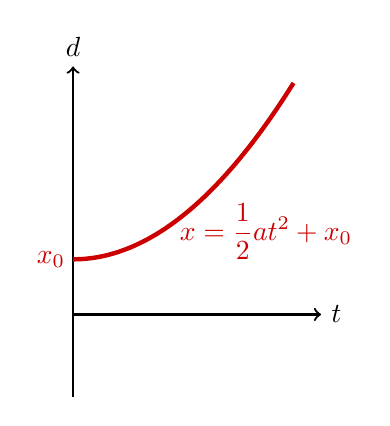
\begin{tikzpicture}[scale=.7]
    \draw[->,thick] (0,0)--(4.5,0) node[right]{$t$};
    \draw[->,thick] (0,-1.5)--(0,4.5) node[above]{$d$};
    \draw[smooth,samples=20,domain=0:4,red!80!black,ultra thick]
    plot({\x},{.2*(\x)*(\x)+1});
    \node[red!80!black] at (3.5,1.5) {$\displaystyle x=\frac12at^2+x_0$};
    \node[red!80!black] at (-.4,1) {$x_0$};
  \end{tikzpicture}
  \hspace{.15in}
  \begin{tikzpicture}[scale=.7]
    \draw[axes] (0,0)--(4.5,0) node[right]{$t^2$};
    \draw[axes] (0,-1.5)--(0,4.5) node[above]{$d$};
    \draw[red!80!black,ultra thick](0,1)--(4,4.2);
    \node[red!80!black] at (3,1.5) {$\displaystyle x=\frac12at^2+x_0$};
    \node[red!80!black] at (-.4,1) {$x_0$};
  \end{tikzpicture}
  \caption{Position plotted against time $t$ and time squared $t^2$ for
    uniformly accelerated motion.}
  \label{switch1}
\end{figure} 


\subsection{Velocity Squared vs.\ Displacement}
Likewise, some experimental equation is able to capture velocity information
as an object moves in \emph{space}. In other words, velocity and position
information is available experimentally but not time. Instead of plotting
velocity vs.\ time, position vs.\ time, we can plot velocity as a function of
\emph{position}. Again, even if acceleration is uniform, finding $a$ from this
graph is not straightforward. However, another option is to, like in the
previous section, re-interpret the kinematic equation as a linear function:
\begin{equation}
  \vertarrowbox{v^2}{$y$}=
  \vertarrowbox{v_0^2}{$b$}+\vertarrowbox{(2a)}{$m$}
  \vertarrowbox{(x-x_0)}{$x$}
\end{equation}
and plot the \emph{square} of velocity $v^2$ as a function of
displacement ($x-x_0$). If acceleration is uniform (constant $a$), the graph
would be linear. The acceleration is half the slope $m$ of the graph:
$a=\dfrac m2$ and the $y$-intercept is the square of the initial velocity
($v_0^2$).


%\subsection{Use of Linear Graphs in Other Applications}
%There are many types of graphs that we plot as linear graphs even though the
%relationship between variables is not linear. In the AP Physics C exams, there
%is often one free-response question where ``experimental'' data is provided for
%a known algebraic relationship, and you as asked to find a constant by plotting
%a linear graph. Some example are shown here.


\subsection{Orbital Mechanics}
The relationship between the period $T$ and orbital radius $R$ of planets
around the same star (Kepler's third law of planetary motion) is most often
shown by plotting $T^2$ vs.\ $R^3$ rather than plotting $T$ vs.\ $R$ directly.
The slope of the graph can be used to find the mass of the star $M$
at the center:
\begin{equation}
  \vertarrowbox{T^2}{$y$}=
  \vertarrowbox{\dfrac{4\pi^2}{GM}}{$m$}
  \vertarrowbox{R^3}{$x$}
\end{equation}



\subsection{Simple Pendulum}
In the simple harmonic motion of a simple pendulum, the relationship between
the frequency $f$ and the length of the pendulum $\ell$ is given
by\footnote{Although \emph{usually} we would write it as
  \begin{equation*}
    f=\frac1{2\pi}\sqrt{\frac \ell{g}}
  \end{equation*}
}
\begin{equation}
  f=\left[\frac1{2\pi\sqrt{g}}\right]\sqrt{\ell}
\end{equation}
In this case, the slope of the graph of $f$ vs.\ $\sqrt\ell$ can be used to
experimentally determine the acceleration due to gravity $g$.



\subsection{Refraction of Light}
In the law of refraction\footnote{You may know it as Snell's law.}, the
incident angle $\theta_1$ and the refracted angle $\theta_2$ when light is
refracted from a vaccuum into a material with refractive index $n$ is given
by:
\begin{equation}
  \vertarrowbox{\sin\theta_1}{$y$}=
  \vertarrowbox{n}{$m$}
  \vertarrowbox{\sin\theta_2}{$x$}
\end{equation}
By plotting $\sin\theta_1$ vs.\ $\sin\theta_2$, we see that the slope of the
graph is the refractive index.
